% Options for packages loaded elsewhere
\PassOptionsToPackage{unicode}{hyperref}
\PassOptionsToPackage{hyphens}{url}
%
\documentclass[
  man,floatsintext]{apa6}
\usepackage{amsmath,amssymb}
\usepackage{iftex}
\ifPDFTeX
  \usepackage[T1]{fontenc}
  \usepackage[utf8]{inputenc}
  \usepackage{textcomp} % provide euro and other symbols
\else % if luatex or xetex
  \usepackage{unicode-math} % this also loads fontspec
  \defaultfontfeatures{Scale=MatchLowercase}
  \defaultfontfeatures[\rmfamily]{Ligatures=TeX,Scale=1}
\fi
\usepackage{lmodern}
\ifPDFTeX\else
  % xetex/luatex font selection
\fi
% Use upquote if available, for straight quotes in verbatim environments
\IfFileExists{upquote.sty}{\usepackage{upquote}}{}
\IfFileExists{microtype.sty}{% use microtype if available
  \usepackage[]{microtype}
  \UseMicrotypeSet[protrusion]{basicmath} % disable protrusion for tt fonts
}{}
\makeatletter
\@ifundefined{KOMAClassName}{% if non-KOMA class
  \IfFileExists{parskip.sty}{%
    \usepackage{parskip}
  }{% else
    \setlength{\parindent}{0pt}
    \setlength{\parskip}{6pt plus 2pt minus 1pt}}
}{% if KOMA class
  \KOMAoptions{parskip=half}}
\makeatother
\usepackage{xcolor}
\usepackage{graphicx}
\makeatletter
\def\maxwidth{\ifdim\Gin@nat@width>\linewidth\linewidth\else\Gin@nat@width\fi}
\def\maxheight{\ifdim\Gin@nat@height>\textheight\textheight\else\Gin@nat@height\fi}
\makeatother
% Scale images if necessary, so that they will not overflow the page
% margins by default, and it is still possible to overwrite the defaults
% using explicit options in \includegraphics[width, height, ...]{}
\setkeys{Gin}{width=\maxwidth,height=\maxheight,keepaspectratio}
% Set default figure placement to htbp
\makeatletter
\def\fps@figure{htbp}
\makeatother
\setlength{\emergencystretch}{3em} % prevent overfull lines
\providecommand{\tightlist}{%
  \setlength{\itemsep}{0pt}\setlength{\parskip}{0pt}}
\setcounter{secnumdepth}{-\maxdimen} % remove section numbering
% Make \paragraph and \subparagraph free-standing
\ifx\paragraph\undefined\else
  \let\oldparagraph\paragraph
  \renewcommand{\paragraph}[1]{\oldparagraph{#1}\mbox{}}
\fi
\ifx\subparagraph\undefined\else
  \let\oldsubparagraph\subparagraph
  \renewcommand{\subparagraph}[1]{\oldsubparagraph{#1}\mbox{}}
\fi
\ifLuaTeX
\usepackage[bidi=basic]{babel}
\else
\usepackage[bidi=default]{babel}
\fi
\babelprovide[main,import]{english}
% get rid of language-specific shorthands (see #6817):
\let\LanguageShortHands\languageshorthands
\def\languageshorthands#1{}
% Manuscript styling
\usepackage{upgreek}
\captionsetup{font=singlespacing,justification=justified}

% Table formatting
\usepackage{longtable}
\usepackage{lscape}
% \usepackage[counterclockwise]{rotating}   % Landscape page setup for large tables
\usepackage{multirow}		% Table styling
\usepackage{tabularx}		% Control Column width
\usepackage[flushleft]{threeparttable}	% Allows for three part tables with a specified notes section
\usepackage{threeparttablex}            % Lets threeparttable work with longtable

% Create new environments so endfloat can handle them
% \newenvironment{ltable}
%   {\begin{landscape}\centering\begin{threeparttable}}
%   {\end{threeparttable}\end{landscape}}
\newenvironment{lltable}{\begin{landscape}\centering\begin{ThreePartTable}}{\end{ThreePartTable}\end{landscape}}

% Enables adjusting longtable caption width to table width
% Solution found at http://golatex.de/longtable-mit-caption-so-breit-wie-die-tabelle-t15767.html
\makeatletter
\newcommand\LastLTentrywidth{1em}
\newlength\longtablewidth
\setlength{\longtablewidth}{1in}
\newcommand{\getlongtablewidth}{\begingroup \ifcsname LT@\roman{LT@tables}\endcsname \global\longtablewidth=0pt \renewcommand{\LT@entry}[2]{\global\advance\longtablewidth by ##2\relax\gdef\LastLTentrywidth{##2}}\@nameuse{LT@\roman{LT@tables}} \fi \endgroup}

% \setlength{\parindent}{0.5in}
% \setlength{\parskip}{0pt plus 0pt minus 0pt}

% Overwrite redefinition of paragraph and subparagraph by the default LaTeX template
% See https://github.com/crsh/papaja/issues/292
\makeatletter
\renewcommand{\paragraph}{\@startsection{paragraph}{4}{\parindent}%
  {0\baselineskip \@plus 0.2ex \@minus 0.2ex}%
  {-1em}%
  {\normalfont\normalsize\bfseries\itshape\typesectitle}}

\renewcommand{\subparagraph}[1]{\@startsection{subparagraph}{5}{1em}%
  {0\baselineskip \@plus 0.2ex \@minus 0.2ex}%
  {-\z@\relax}%
  {\normalfont\normalsize\itshape\hspace{\parindent}{#1}\textit{\addperi}}{\relax}}
\makeatother

% \usepackage{etoolbox}
\makeatletter
\patchcmd{\HyOrg@maketitle}
  {\section{\normalfont\normalsize\abstractname}}
  {\section*{\normalfont\normalsize\abstractname}}
  {}{\typeout{Failed to patch abstract.}}
\patchcmd{\HyOrg@maketitle}
  {\section{\protect\normalfont{\@title}}}
  {\section*{\protect\normalfont{\@title}}}
  {}{\typeout{Failed to patch title.}}
\makeatother

\usepackage{xpatch}
\makeatletter
\xapptocmd\appendix
  {\xapptocmd\section
    {\addcontentsline{toc}{section}{\appendixname\ifoneappendix\else~\theappendix\fi\\: #1}}
    {}{\InnerPatchFailed}%
  }
{}{\PatchFailed}
\keywords{systematicity, phonological development, preferential attachment, networks analysis}
\usepackage{csquotes}
\usepackage[titles]{tocloft}
\cftpagenumbersoff{figure}
\renewcommand{\cftfigpresnum}{\itshape\figurename\enspace}
\renewcommand{\cftfigaftersnum}{.\space}
\setlength{\cftfigindent}{0pt}
\setlength{\cftafterloftitleskip}{0pt}
\settowidth{\cftfignumwidth}{Figure 10.\qquad}
\DeclareDelayedFloatFlavor{kableExtra}{table}
\usepackage{tipa}
\ifLuaTeX
  \usepackage{selnolig}  % disable illegal ligatures
\fi
\IfFileExists{bookmark.sty}{\usepackage{bookmark}}{\usepackage{hyperref}}
\IfFileExists{xurl.sty}{\usepackage{xurl}}{} % add URL line breaks if available
\urlstyle{same}
\hypersetup{
  pdftitle={Systematicity over the course of early development: an analysis of phonological networks: Supplementary materials},
  pdfauthor={Catherine E. Laing1},
  pdflang={en-EN},
  pdfkeywords={systematicity, phonological development, preferential attachment, networks analysis},
  hidelinks,
  pdfcreator={LaTeX via pandoc}}

\title{Systematicity over the course of early development: an analysis of phonological networks: Supplementary materials}
\author{Catherine E. Laing\textsuperscript{1}}
\date{}


\shorttitle{Network graphs of early phonological development}

\authornote{

All code and associated data for this manuscript can be found at \url{https://github.com/cathelaing/NetworkGraphs}. Data provided in the PhonBank corpus was collected through support from grant number NIH-NICHHD RO1-HD051698.

Correspondence concerning this article should be addressed to Catherine E. Laing, Department of Language and Linguistic Science, University of York, Heslington, YO10 5DD.. E-mail: \href{mailto:catherine.laing@york.ac.uk}{\nolinkurl{catherine.laing@york.ac.uk}}

}

\affiliation{\vspace{0.5cm}\textsuperscript{1} University of York, York, UK}

\begin{document}
\maketitle

\hypertarget{s1-testing-model-fit}{%
\subsection{S1: Testing model fit}\label{s1-testing-model-fit}}

Nested model comparisons were initially used to establish the best model fit for the data without the inclusion of Data type. Model comparisons testing Network size (\emph{numNodes in the model}) are shown below. Including Network size alongside Age improved model fit for all models except the initial model testing mean path length.

\hypertarget{mean-path-length}{%
\subsubsection{Mean Path Length}\label{mean-path-length}}

\begin{verbatim}
## Data: subset(SWD_red, data_type %in% c("actual", "WS_actual", "Erdos_Renyi"))
## Models:
## MPL.0: path_length ~ corpus + age + (1 + age | Speaker)
## MPL.1: path_length ~ corpus + age + numNodes + (1 + age | Speaker)
##       npar    AIC    BIC  logLik deviance  Chisq Df Pr(>Chisq)
## MPL.0    7 1039.0 1067.5 -512.49   1025.0                     
## MPL.1    8 1040.7 1073.2 -512.36   1024.7 0.2726  1     0.6016
\end{verbatim}

\hypertarget{clustering-coefficient}{%
\subsubsection{Clustering coefficient}\label{clustering-coefficient}}

\begin{verbatim}
## Data: subset(SWD_red, data_type %in% c("actual", "WS_actual", "Erdos_Renyi"))
## Models:
## CC.0: clust_coef_avg ~ corpus + age + (1 + age | Speaker)
## CC.1: clust_coef_avg ~ corpus + age + numNodes + (1 + age | Speaker)
##      npar    AIC    BIC  logLik deviance  Chisq Df Pr(>Chisq)    
## CC.0    7 376.71 405.17 -181.35   362.71                         
## CC.1    8 367.79 400.32 -175.90   351.79 10.916  1  0.0009535 ***
## ---
## Signif. codes:  0 '***' 0.001 '**' 0.01 '*' 0.05 '.' 0.1 ' ' 1
\end{verbatim}

\hypertarget{data-type-mean-path-length}{%
\subsubsection{Data type: Mean path length}\label{data-type-mean-path-length}}

\begin{verbatim}
## Data: subset(SWD_red, data_type %in% c("actual", "target"))
## Models:
## MPL.DT.0: path_length ~ corpus + age + (1 + age | Speaker)
## MPL.DT.1: path_length ~ corpus + age + numNodes + (1 + age | Speaker)
##          npar     AIC     BIC logLik deviance  Chisq Df Pr(>Chisq)    
## MPL.DT.0    7 -100.59  -74.83 57.296  -114.59                         
## MPL.DT.1    8 -147.18 -117.74 81.589  -163.18 48.586  1  3.161e-12 ***
## ---
## Signif. codes:  0 '***' 0.001 '**' 0.01 '*' 0.05 '.' 0.1 ' ' 1
\end{verbatim}

\hypertarget{data-type-clustering-coefficient}{%
\subsubsection{Data type: Clustering coefficient}\label{data-type-clustering-coefficient}}

\begin{verbatim}
## Data: subset(SWD_red, data_type %in% c("actual", "target"))
## Models:
## CC.DT.0: clust_coef_avg ~ corpus + age + (1 + age | Speaker)
## CC.DT.1: clust_coef_avg ~ corpus + age + numNodes + (1 + age | Speaker)
##         npar     AIC     BIC logLik deviance  Chisq Df Pr(>Chisq)    
## CC.DT.0    7 -539.31 -513.55 276.65  -553.31                         
## CC.DT.1    8 -578.48 -549.04 297.24  -594.48 41.168  1  1.397e-10 ***
## ---
## Signif. codes:  0 '***' 0.001 '**' 0.01 '*' 0.05 '.' 0.1 ' ' 1
\end{verbatim}

\hypertarget{s2-running-figures-with-age-instead-of-network-size}{%
\subsection{S2: Running figures with Age instead of Network size}\label{s2-running-figures-with-age-instead-of-network-size}}

In the main paper, figures showing change in mean path length and clustering coefficient are visualised in relation to changing network size. Figures \ref{fig:Figure-path-length-age}-\ref{fig:Figure-clust-coef-DT-age} plot the same data according to Age in months.

\begin{figure}
\centering
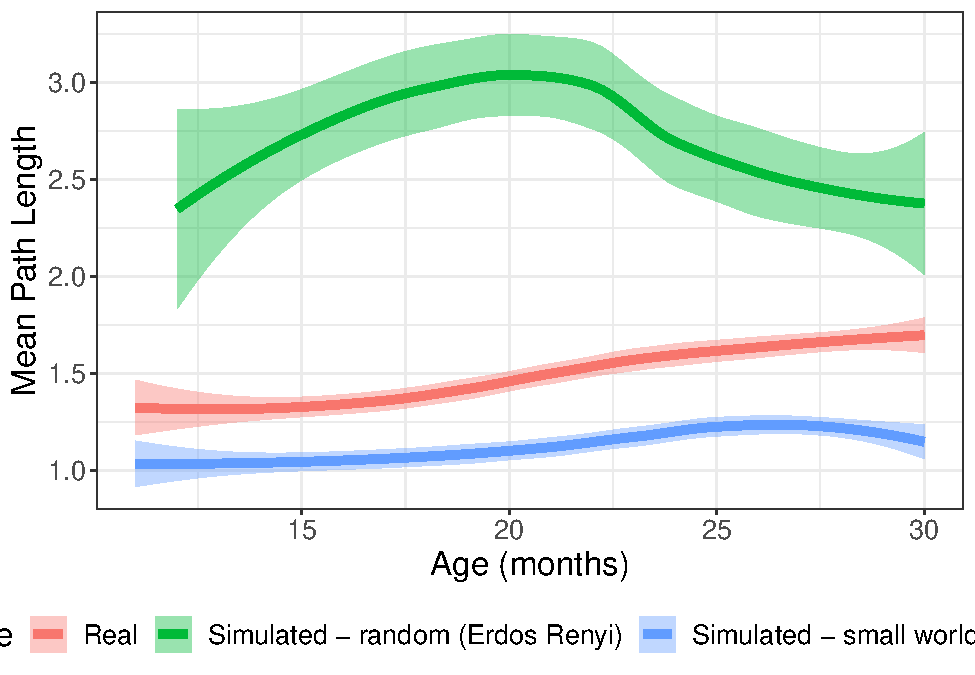
\includegraphics{NetworkGraphs_supplementary-data_files/figure-latex/Figure-path-length-age-1.pdf}
\caption{\label{fig:Figure-path-length-age}Change in mean path length over time, in Real data (Actual) compared with Simulated small-world (Watts-Strogatz) and random (Erdos--Rényi) networks. Coloured lines represent Data type; coloured bands represent 95\% CIs.}
\end{figure}

\begin{figure}
\centering
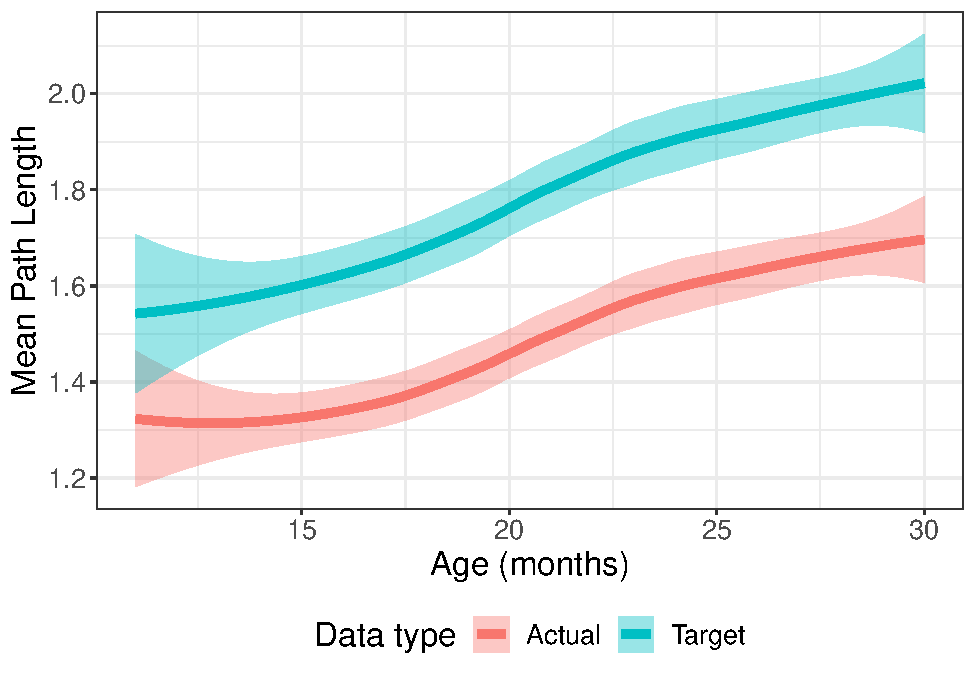
\includegraphics{NetworkGraphs_supplementary-data_files/figure-latex/Figure-path-length-DT-age-1.pdf}
\caption{\label{fig:Figure-path-length-DT-age}Change in mean path length over time, in Actual vs.~Target data. Coloured lines represent Data type; coloured bands represent 95\% CIs.}
\end{figure}

\begin{figure}
\centering
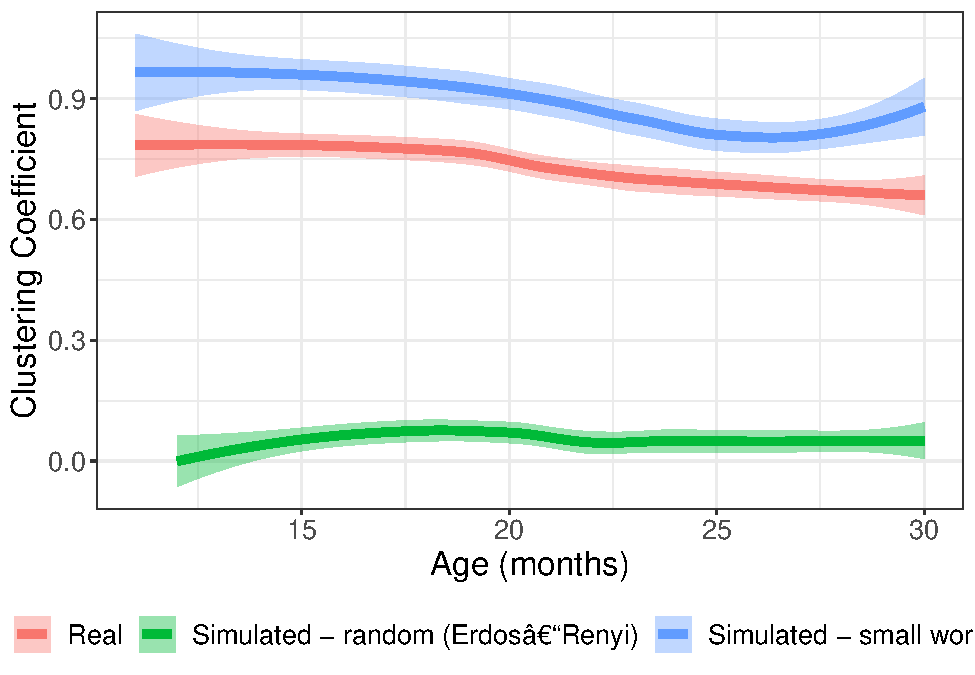
\includegraphics{NetworkGraphs_supplementary-data_files/figure-latex/Figure-clust-coef-age-1.pdf}
\caption{\label{fig:Figure-clust-coef-age}Change in mean clustering coefficient over time, in Real data (Actual) compared with Simulated small-world (Watts-Strogatz) and random (Erdos--Rényi) networks. Coloured lines represent Data type; coloured bands represent 95\% CIs.}
\end{figure}

\begin{figure}
\centering
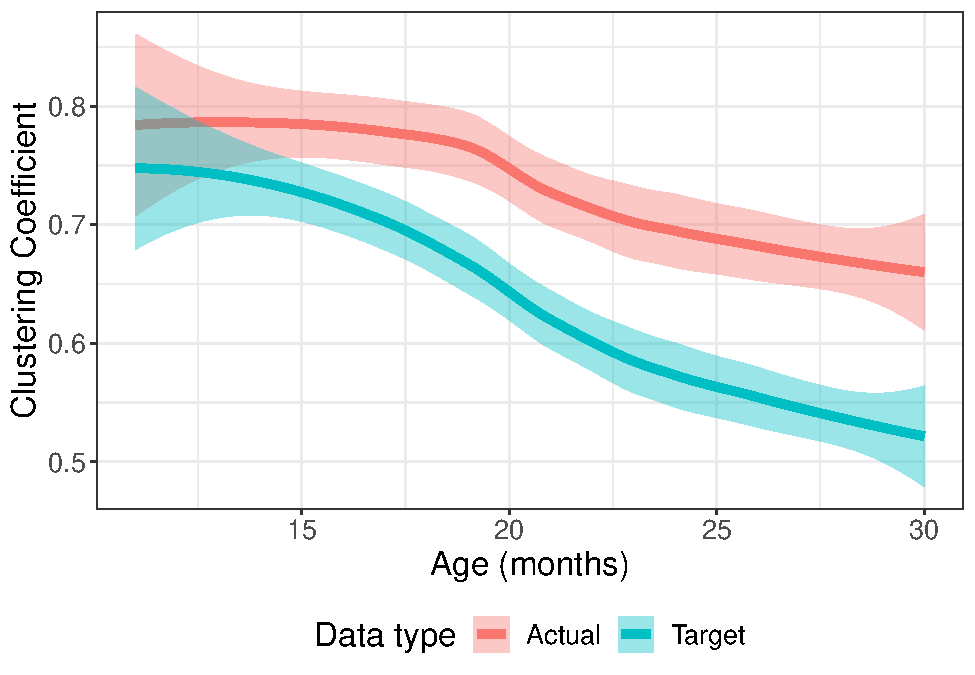
\includegraphics{NetworkGraphs_supplementary-data_files/figure-latex/Figure-clust-coef-DT-age-1.pdf}
\caption{\label{fig:Figure-clust-coef-DT-age}Change in mean clustering coefficient over time, in Actual vs.~Target data. Coloured lines represent Data type; coloured bands represent 95\% CIs.}
\end{figure}


\clearpage
\renewcommand{\listfigurename}{Figure captions}


\end{document}
